% Document template suitable for use as a LaTeX master-file 
% for thesis works in University of Turku Department of Computing
%
% Technical usage guide: https://tech.utugit.fi/soft/thesis/doc/doc/overview/
% 

\documentclass[language=finnish,version=final,mainfont=none,sharelatex=false]{utuftthesis}
\setcounter{secnumdepth}{2}
\setcounter{tocdepth}{2}
\usepackage{float}
\usepackage[caption=false]{subfig}

% Define the algorithm environment
%\makeatletter
\providecommand\textquotedblplain{%
  \bgroup\addfontfeatures{Mapping=}\char34\egroup}
\providecommand{\tabularnewline}{\\}
\floatstyle{ruled}
\newfloat{algorithm}{tbp}{loa}
\providecommand{\algorithmname}{Algoritmi}
\floatname{algorithm}{\protect\algorithmname}
%\makeatother

\addbibresource{Bibliografia.bib}

\begin{document}

\pubyear{2023}
\pubmonth{2}
\publab{Labran nimi}
\publaben{Laboratory Name}
\pubtype{tkk}
\title{Polunetsintäalgoritmit (väliaikainen otsikko)}
\author{Botond Ortutay}

\maketitle
\keywords{algoritmiikka, polunetsintä, graafiteoria}

\keywordsen{algorithmics, path finding, graph theory}
\begin{abstract}
\textit{Tässä tutkielmassa tarkastellaan polunetsintäalgoritmeja koneellisen 
polunetsinnän näkökulmasta. Tutkielma on kirjallisuuskatsaus, eli se perustuu 
pääosin aiheesta julkaistuun tieteelliseen kirjallisuuteen, mutta se sisältää 
pienimuotoisen tutkimuksen eräiden algoritmien mittaamisesta 
testiympäristössä. Tutkielma esittellee lukijalle joitakin 
polunetsintäalgoritmeja, sekä niiden käyttökohteita ja vertailee niiden 
tehokkuutta.}
\end{abstract}

\begin{abstracten}
\textit{This thesis examines path finding algorithms from a computing 
oriented point of view. It is a literature review, so it is mostly based on 
already published research. It also contains a small set of performance 
measurements of certain algorithms in a test environment. The thesis 
introduces the reader to a few path finding algorithms, their use cases and 
it compares their performance.}
\end{abstracten}



% mandatory
\tableofcontents

% if you want a list of figures
\listoffigures

% if you want a list of tables
\listoftables

% if you want a list of acronyms
\listofacronyms

% change the name if the default doesn't sound right
\renewcommand{\algorithmname}{\listingscaption}

% The thesis starts here.

\begin{comment}
To better organize things, create a new tex file for each chapter
and input it below.

Avoid using the å, ä, ö or <space> characters in referred names and
underscores \_ in file names (may break hyperref).

Good luck!
\end{comment}

\chapter{Johdanto} \label{Johdanto}

\section{Tutkielman tarkoitus}\label{tTarkoitus}
\begingroup
\itshape
\paragraph{*Suunnitelma kappaleelle 1.1:*}
\begin{itemize}
	\item Harkittu ja kiinnostava aloitus
	\item Käy lyhyesti ja yksinkertaisesti läpi seuraavat asiat:
	\begin{itemize}
		\item Polunetsintäalgoritmejä tarvitaan kun...
		\item Polunetsintä käsitteenä
		\item Miski kirjoitin kandityön juuri tästä aiheesta? (tutkielman perustelu)
	\end{itemize}
	\item Päätä kappale jotenkin näin:
\end{itemize}
"Tutkielman tarkoitus on esitellä lukijalle erilaisia polunetsintäalgoritmeja, 
sekä verrata niiden toimintaa jossakin esimerkkiympäristössä"
\endgroup

\section{Tutkimuskysymykset}\label{tutkimuskysymykset}
Tutkielmassa pyritöön vastaamaan seuraaviin kysymyksiin:
\begin{enumerate}[label=\textbf{\arabic*.}]
	\item \label{tKysymys1} \textbf{Tutkimuskysymys:} Minkälaisia polunetsintäalgoritmeja on kehitetty?
	\item \label{tKysymys2} \textbf{Tutkimuskysymys:} Miten niitä voidaan käyttää käytännön sovelluksiin?
	\item \label{tKysymys3} \textbf{Tutkimuskysymys:} Miten niiden tehokkuutta voidaan mitata?
\end{enumerate}

\section{Tiedonhakumenetelmät}\label{tiedonhakuM}
Tietoa tämän tutkielman tekoon on haettu IEEE:n Xplore Digital 
Center-tietokannasta, Web of Science-tietokannasta, sekä Google 
Scholar-hakupalvelusta. Hakutuloksia rajattiin julkaisuajan mukaan niin, 
että suurin osa hakutuloksista on julkaistu vuona 2018 tai sen jälkeen. 
Myös aihepiirirajausta on käytetty. Hakusanoissa on käytetty osuvempien 
tulosten löytämiseksi Boolen operaattoreita, sekä sanakatkaisua. Alla on 
muutama esimerkki käytetyistä hakusanoista:
\begin{center}
\texttt{
	pathfinding AND (grid based OR graph theory) AND "map*"	\\
	"pathfinding" AND "video gam*"				\\
	comparing AND "pathfinding algorithms"			\\
}
\end{center}

\section{Tutkielman rakenne}\label{tRakenne}
Tutkielman luku \ref{Taustoitus} taustoittaa seuraavia lukuja. Tarkoitus on, 
että luvun \ref{Taustoitus} lukemisen jälkeen lukijalle tulisivat tutuksi 
polunetsintään liittyvät peruskäsitteet ja tausta-aiheet, jotta seuraavien 
lukujen ymmärtäminen helpottuisi. Luvussa \ref{joitainP} käydään läpi 
muutaman tunnetun polunetsinnän toiminta ja täten pyritään vastaamaan 
tutkimuskysymykseen \ref{tKysymys1} Luvussa 
\ref{algoritmienSovelluskohteita} käydään läpi joitakin 
polunetsintäaldoritmien yleisiä käyttökohteita ja pyritään vastaamaan 
tutkimuskysymykseen \ref{tKysymys2} Luvussa \ref{benchmarking} taas mitataan 
useiden eri polunetsintäalgoritmien tehokkuus eräässä esimerkkiongelmassa ja 
vertaillaan niitä tämän avulla toisiinsa. Lopussa olevassa 
yhteenvetokappaleessa \ref{yhteenveto} tulokset kootaan vielä yhteen ja 
esitetään helpommin luettavassa muodossa.
\chapter{Toisen luvun otsikko} \label{Toinen luku}

Tässä luvussa tarkastellaan kahden kuvan upottamista samaan kelluvaan
kuvaympäristöön (Kuva \ref{fig:Optimointia-kahdella-eri}).

\begin{figure}[tbh]
\subfloat[Käynnistysajan optimointi Nailgunilla.]{\begin{centering}
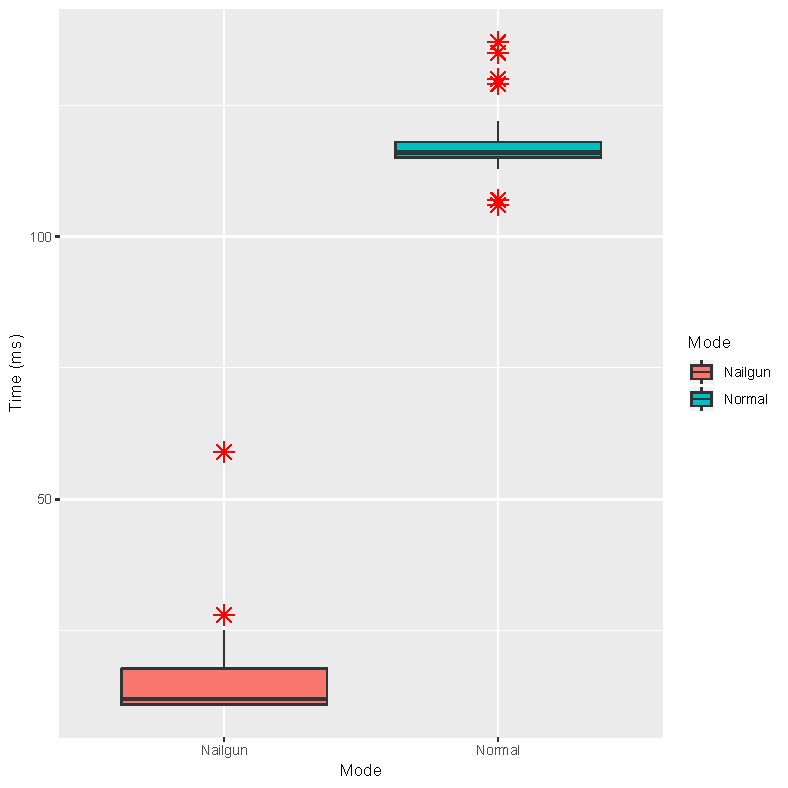
\includegraphics[width=0.45\textwidth]{kuvat/nailgun.pdf}
\par\end{centering}
}\subfloat[Koon optimointi Proguardilla.]{\begin{centering}
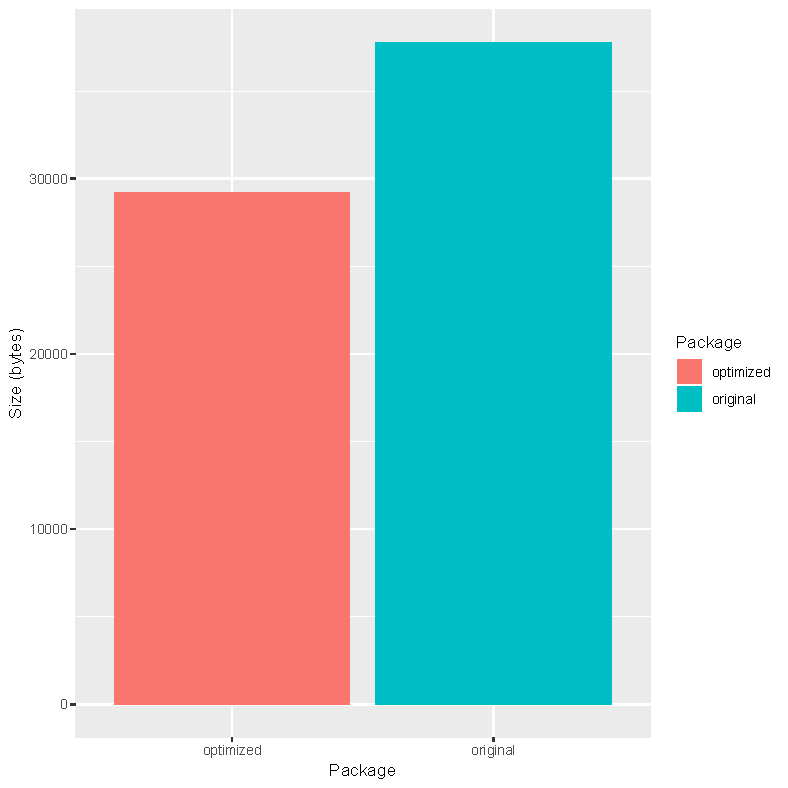
\includegraphics[width=0.45\textwidth]{kuvat/proguard.pdf}
\par\end{centering}
}\caption{Optimointia kahdella eri tavalla.\label{fig:Optimointia-kahdella-eri}}

\end{figure}



%\input{file_name_of_chapter_x}
%\input{file_name_of_chapter_y}

% The thesis main content ends here.

\printbibliography

\begin{comment}
Important! Create the appendix chapters with command \textbackslash appchapter\{some
name\} instead of \textbackslash chapter\{some name\} for the automagic
page counting to work!
\end{comment}


\appchapter{Liitedokumentti}

Liitteen ohjelmakoodi \ref{alg:Tyyppiluokka-Monad} kuvaa matemaattisen
monadirakenteen pohjalta rakentuvan Haskellin tyyppiluokan. Tyyppiluokan
voi nähdä eräänlaisena abstraktina ohjelmointirajapintana (API\nomenclature[API]{API}{Application Programming Interface}),
joka muodostaa ohjelmoijalle abstraktin ohjelmointikielen käyttöliittymän
(UI\nomenclature[UI]{UI}{User Interface}).

\begin{algorithm}[tbh]
\begin{minted}{haskell}
class Monad m where
    ( >>= )         :: m a -> (a -> m b) -> m b
    return          :: a                 -> m a

    fail            :: String            -> m a
    (>>)            :: m a -> m b        -> m b
    m >> k          =  m >>= \_ -> k       -- default

instance Monad IO where  ...               -- omitted
\end{minted}

\caption{Tyyppiluokka 'Monad'.\label{alg:Tyyppiluokka-Monad}}
\end{algorithm}

\newpage{}

Ensimmäisen liitteen toinen sivu. Ohjelmalistaus \ref{alg:Monadin-kayttoa}
demonstroi vielä monadin käyttöä.

\begin{algorithm}[tbh]
\begin{minted}{haskell}
main =
return "Your name:" >>=
putStr >>=
\_ -> getLine >>=
\n -> putStrLn ("Hey " ++ n)
\end{minted}

\caption{Monadin käyttöä.\label{alg:Monadin-kayttoa}}
\end{algorithm}


\appchapter{Liitedokumentti 2}

Tässä esimerkki\pagebreak{}

toisesta kaksisivuisesta liitteestä.
\end{document}
